\documentclass[]{article}

\usepackage[pdftex]{graphicx}
% Title Page
\title{Group Project Proposal: Race the Wild}
\author{}


\begin{document}
\maketitle

We have been tasked with using animal tracking data, as well as tracking via smartphone to produce an application that educates about animals. The following proposal is an idea that aims to blend these with a product people will find appealing to use.

The basic premise of the idea is having the app running on a smartphone monitoring movement via satellite navigation, to approximate distance travelled. The idea is that can be compared with the movements of animals, for which data will be stored with the app.


\begin{center}

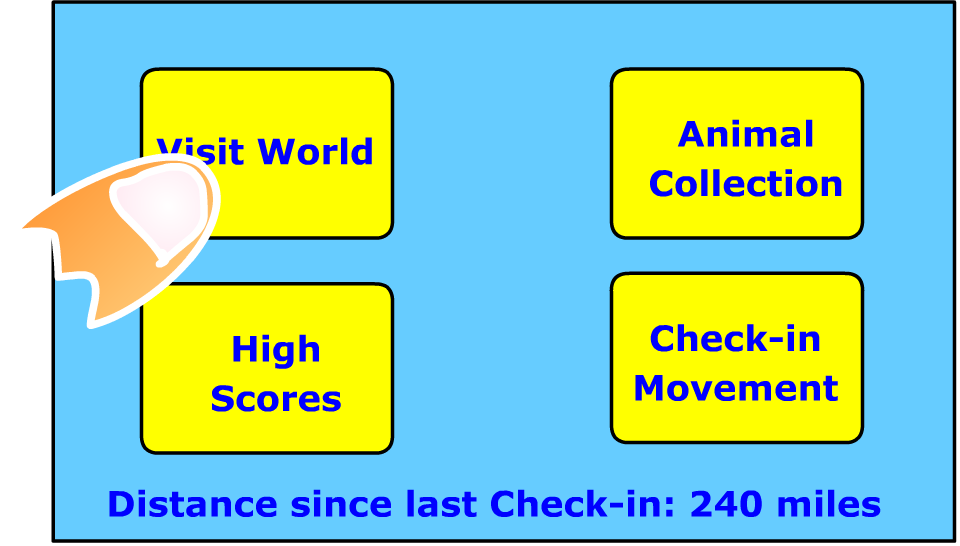
\includegraphics[scale=0.2]{menu.png}

Fig.1: a mock-up of the main menu


\end{center}

By ``checking in'' with the application, users can collect new animals to find in a virtual world inside the application. To allow them to move inside this virtual world, by checking in users will receive movement points based on how far they have travelled, which will allow them to move between various habitats to find animals. The goal of this is not for people to drive around to receive points, so one idea is to track movement velocities and reward more points for behaviour which appears to be walking or cycling.

\begin{center}

\includegraphics[scale=0.2]{checkin.png}

Fig.2: A mock-up of the check-in screen

\end{center}

The idea is that the world map will be presented as a simple touch based graph interface, with costs for moving between nodes. The end user, once an animal is available to find, will have to guess / work out which habitat the animal is most suited to (perhaps via research), and then can move to the correct location to find it.

\begin{center}
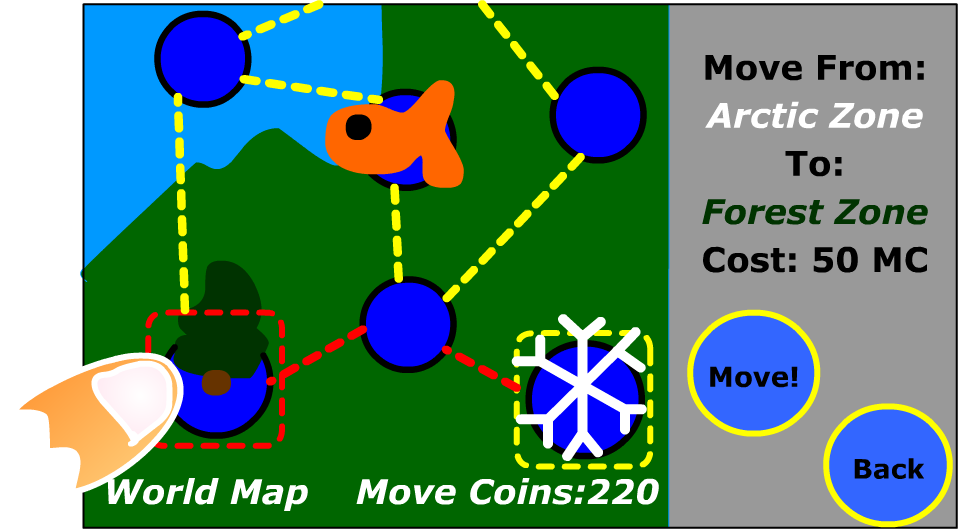
\includegraphics[scale=0.22]{worldmap.png}

Fig. 3: The world map mock-up.
\end{center}

\begin{center}
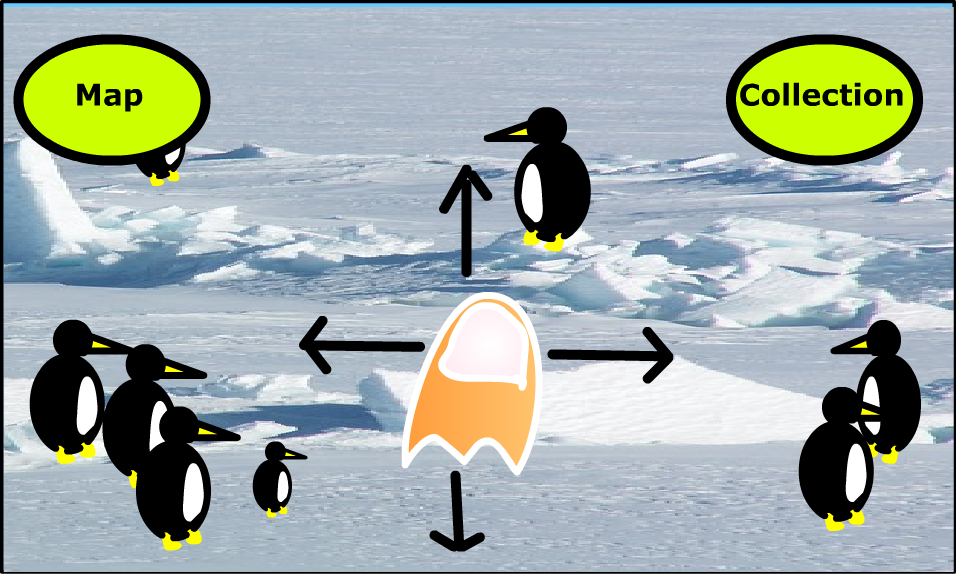
\includegraphics[scale=0.22]{zone1.png}

Fig. 4: a touch based interface for the world map
\end{center}

Once in a location, the user can scroll around it using a touch interface, in an attempt to find any animals they have been compared to but have not yet found. Animals which have already been found will also be in the area, to give the game a slight difficulty curve, and by touching the new animal once found, it can be added to the collection. Note: the animals in this scene are for illustration of the concept, rather than for illustrating actual habitats.

\begin{center}
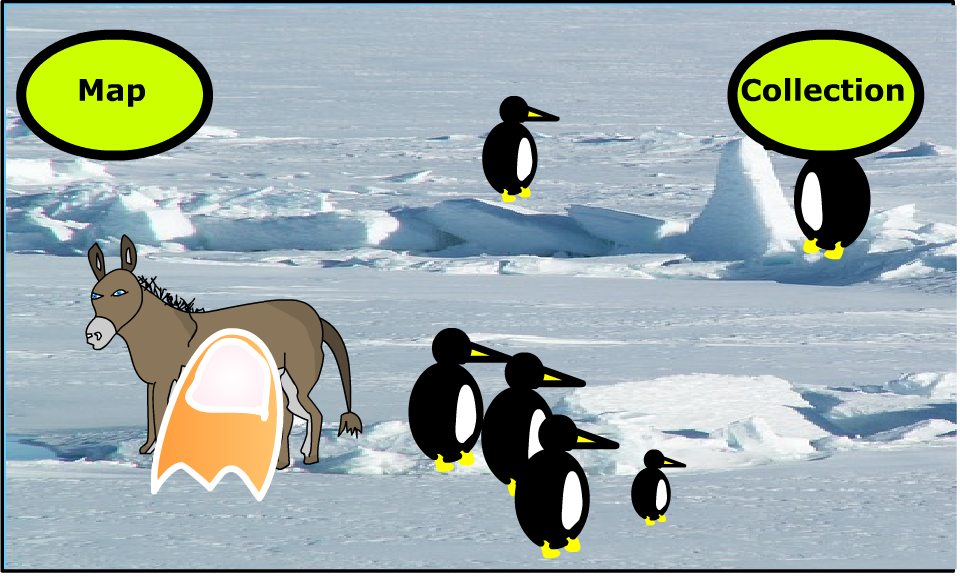
\includegraphics[scale=0.22]{zone2.png}

Fig. 5: A scrolled version of Fig. 4
\end{center}

As a reward for finding an animal, the user will be presented with various facts about it, as well as the thrill of having collected something. An online high score system could also be developed, so that the person who finds the most animals / gains the most movement points could rise to the top of this.

\begin{center}
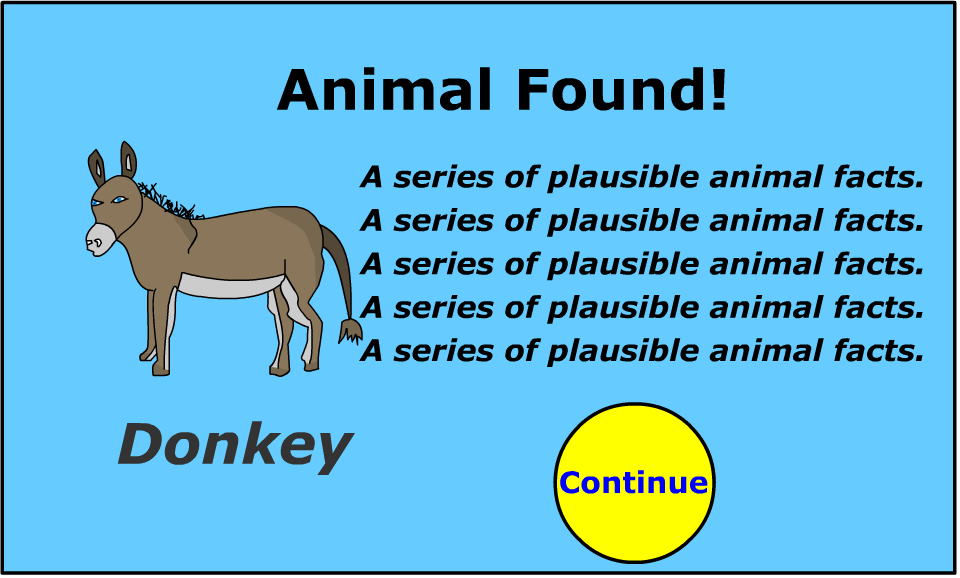
\includegraphics[scale=0.22]{animalfound.png}

Fig. 6: An information screen.
\end{center}

To see their progress, or find information on animals they have encountered via walking but are yet to find in the game, the user can visit the collection screen. This will give them access to this information, as well as the facts they have collected about each animal. This will also be navigable by a scrolling touch interface.

\begin{center}
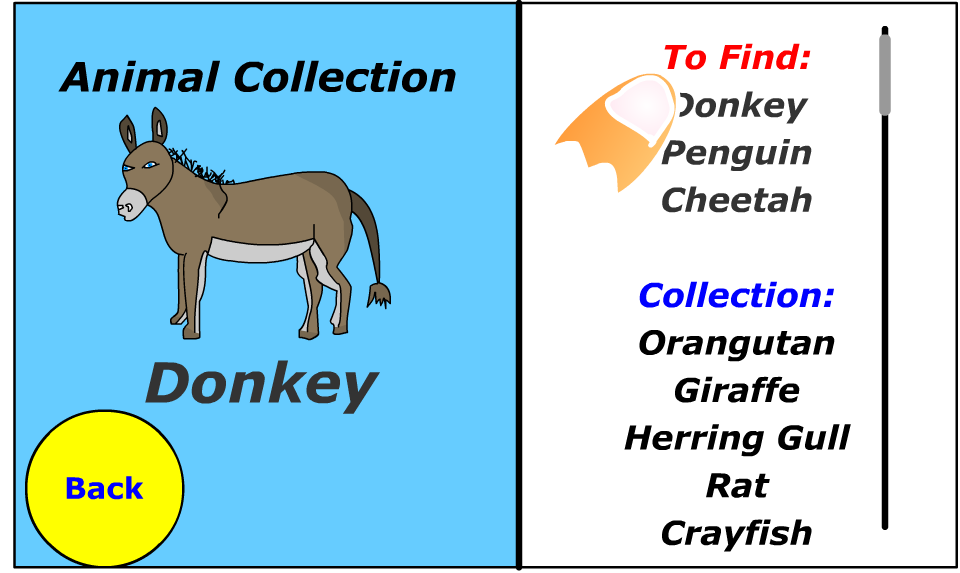
\includegraphics[scale=0.22]{collection.png}

Fig. 6: The collection.
\end{center}

Possible extensions to the project are a separate application to add new animals to the program via a simple PC graphical user interface, and perhaps a mission based system to, for example, find food for animals in the user's collection, to educate on the diets of animals. The project is also ripe for extension based on other data we may receive, provided it can integrate well with the rest of the design.


\end{document}          
